\documentclass[12pt]{article}
\usepackage[utf8]{inputenc}
\usepackage{geometry}
\usepackage{graphicx}
\usepackage{amsmath}
\usepackage{amssymb}
\usepackage{hyperref}
\usepackage{titlesec}
\usepackage{fancyhdr}
\usepackage{enumitem}
\usepackage{xcolor}
\usepackage{caption}
\usepackage{subcaption}
\usepackage{float}

% Page geometry
\geometry{a4paper, margin=1in}

% Header and footer
\pagestyle{fancy}
\fancyhf{}
\fancyhead[L]{\nouppercase{\leftmark}}
\fancyhead[R]{Federated Learning}
\fancyfoot[C]{\thepage}
\renewcommand{\headrulewidth}{0.4pt}
\renewcommand{\footrulewidth}{0.4pt}

% Section formatting
\titleformat{\section}{\large\bfseries}{\thesection}{1em}{}
\titleformat{\subsection}{\normalsize\bfseries}{\thesubsection}{1em}{}

% Custom commands
\newcommand{\W}{\mathcal{W}}
\newcommand{\Lk}{\mathcal{L}_k}
\newcommand{\Dk}{\mathcal{D}_k}

\begin{document}

% Title Page
\begin{titlepage}
    \centering
    \vspace*{1cm}
    
    % Top
    {\Huge \textbf{UNIVERSITY OF CALCUTTA}}\\[1.5cm]
    
    % Center
    \vfill
    
    {\LARGE \textbf{Federated Learning}}\\[0.5cm]
    {\large M.Sc. Semester III}\\[0.3cm]
    {\large Paper Code: CSMP-306}\\[0.3cm]
    {\large Session: 2025-26}\\[1cm]
    
    {\large \textbf{Submitted By}}\\[0.2cm]
    {\large Debottam Kar}\\[0.2cm]
    {\large CU Roll: C91/CSC/241011}\\[0.2cm]
    {\large Reg. No: 313-1111-0359-21}
    
    \vfill
    
    % Bottom
    {\large }
    
    \vspace*{1cm}
\end{titlepage}

% Index
\tableofcontents
\newpage

% Introduction
\section{Introduction: What is Federated Learning?}
\label{sec:intro}

Healthcare has evolved significantly with the integration of technology, enabling processes like patient registration, remote monitoring, and self-care applications. The rise of the Internet of Medical Things (IoMT) has dramatically increased the volume of digital health data, and Artificial Intelligence (AI) is now used to analyse this data for applications like disease prognosis and personalized care.

However, this growth brings serious challenges around data privacy and security. Healthcare organizations handle vast amounts of sensitive patient information — medical records, diagnoses, treatment histories — and protecting this data from breaches has become a critical concern.

Deep learning (DL), a powerful branch of AI, plays a dual role in this landscape: it helps to analyse patient data for disease diagnosis and treatment planning, while also strengthening cybersecurity defence against threats and fraud in healthcare systems.

To address the tension between data utility and privacy, Federated Learning (FL) has emerged as a promising solution. Rather than centralizing raw patient data, FL trains machine learning models directly on decentralized sources — individual hospitals, clinics, or patient devices — and shares only model updates with a central server. This keeps sensitive data localized and secure. FL systems are built around three core components: client devices, a federated server, and a communication protocol.

In essence, the text frames federated learning as a natural response to the growing need for privacy-preserving AI in an increasingly data-driven healthcare environment.

Federated learning is a machine learning approach where multiple devices or organizations collaboratively train a shared model without sharing their raw data.

Instead of sending data to a central server, each participant:
\begin{enumerate}
    \item Downloads the current global model.
    \item Trains it locally on their own data.
    \item Sends only the updated model parameters (not the data) back to a central server.
    \item The server aggregates all updates to improve the global model.
    \item The process repeats.
\end{enumerate}

\section{Traditional Machine Learning vs Federated Learning}
\label{sec:comparison}

In traditional approaches, all data is collected in one place and used to train a model.
\begin{itemize}
    \item Data from multiple sources is sent to a central server
    \item The model is trained on this centralized dataset
    \item After training, the model is deployed
\end{itemize}
\textbf{Example:} A company collects all user data (images, text, transactions) on its servers and trains a model there.

\subsection{Key Characteristics}
\begin{itemize}
    \item Centralized data storage
    \item Easier to manage and train
    \item Requires moving data to one location
    \item Higher risk of data breaches
    \item Huge Bandwidth usage (Huge data transfer)
\end{itemize}

\begin{figure}[H]
    \centering
    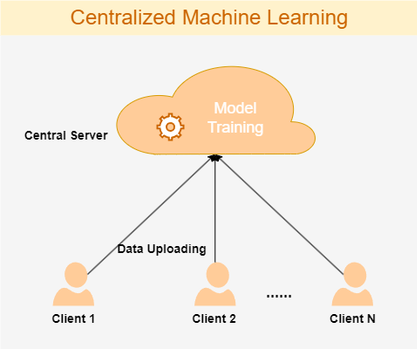
\includegraphics[width=0.7\textwidth]{2.png} % Replace with actual figure
    \caption{Centralized Machine Learning}
    \label{fig:centralized}
\end{figure}

Federated learning trains a model across multiple devices without collecting raw data.
\begin{itemize}
    \item Data stays on local devices (phones, hospitals, banks, etc.)
    \item Each device trains the model locally
    \item Only model updates (not data) are shared with a central server
    \item The server aggregates updates to improve the global model
\end{itemize}
\textbf{Example:} Your phone improves a keyboard prediction model using your typing data—without sending your messages anywhere.

\subsection{Key Characteristics}
\begin{itemize}
    \item Decentralized data
    \item Stronger privacy protection
    \item Data never leaves the device
    \item More complex training process
\end{itemize}

\begin{figure}[H]
    \centering
    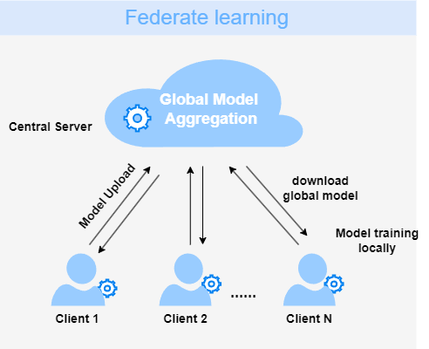
\includegraphics[width=0.7\textwidth]{3.png} % Replace with actual figure
    \caption{Federated Learning Architecture}
    \label{fig:federated}
\end{figure}

\section{Federated Learning in Depth}
\label{sec:in_depth}

\subsection{Core Idea}
Instead of bringing data to the model, Federated Learning brings the model to the data.
\begin{itemize}
    \item Each client (device/organization) keeps its local dataset
    \item A shared global model is collaboratively trained
    \item Only model updates (gradients or weights) are exchanged
\end{itemize}

\subsection{System Architecture}

\begin{figure}[H]
    \centering
    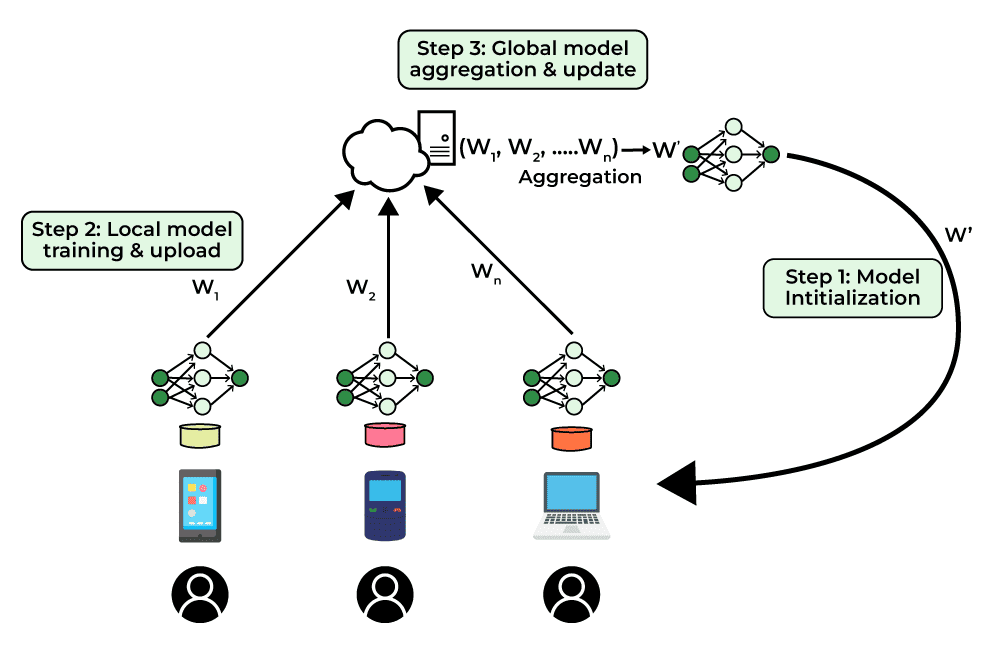
\includegraphics[width=0.9\textwidth]{4.png} % Replace with actual figure
    \caption{Federated Learning System Architecture}
    \label{fig:architecture}
\end{figure}

\subsubsection{Participants}

\textbf{Server (Coordinator):} \\
The server maintains the global model and is responsible for orchestrating the entire training process. It selects which clients participate in each round, distributes the current model to them, and aggregates their updates to produce an improved global model. It never sees raw data — only model updates.

\textbf{Clients (Edge Devices)} \\
Clients are the data-holding participants: smartphones, hospitals, banks, IoT sensors, etc. Each client trains the shared model on its own local data and sends only the resulting weight updates back to the server. Raw data never leaves the device.

\subsubsection{Training Workflow}

\textbf{Step 1: Server initializes the global model} \\
The server randomly initializes a global model $\W_0$ (using Gaussian, Xavier, or He initialization). This defines the shared architecture for all participants. A round counter $t$ is set to 0.

\textbf{Step 2: Server selects a subset of clients} \\
At the start of each round $t$, the server selects a random subset of $C \cdot |S|$ clients (where $C$ is the participation fraction, typically 10–30\%). Selection can be uniform or weighted by data volume. Non-selected clients remain idle for that round.

\textbf{Step 3: Server broadcasts the current model} \\
The current global weights $\W_t$ are sent to every selected client. In practice, weights are compressed or quantized before transmission to reduce communication cost.

\textbf{Step 4: Clients train locally on private data} \\
Each selected client runs $E$ epochs of mini-batch gradient descent on its local dataset $\Dk$, starting from the received $\W_t$. The local gradient is computed as:
\[
\nabla L(\W; x_i, y_i) \quad \text{--- evaluated only on local samples}
\]
The resulting local model becomes:
\[
\W_k^{(t+1)} = \W_t - \eta \cdot \nabla L_k(\W_t)
\]
Only the weight delta $\Delta \W_k$ is prepared for upload. No raw data is transmitted.

\textbf{Step 5: Clients upload updates; server aggregates} \\
Each selected client sends its $\Delta \W_k$ (or full $\W_k^{(t+1)}$) to the server. The server applies the FedAvg algorithm:
\[
\W_{t+1} = \sum \frac{n_k}{n} \cdot \W_k^{(t+1)}
\]
This is a weighted average across clients, where $n_k$ is the number of local samples on client $k$ and $n$ is the total samples across all participating clients. The new global model implicitly reflects learning from all clients' private data without the server ever seeing it.

The round counter increments to $t+1$ and the cycle repeats until convergence.

\subsection{Key Design Considerations}

\begin{itemize}
    \item \textbf{FedAvg weighting:} clients with more data exert proportionally greater influence on the global model. A hospital with 10,000 records contributes more than a phone with 500.
    
    \item \textbf{Communication efficiency:} Gradient sparsification, quantization (8-bit vs. 32-bit floats), and sketching can reduce communication cost by 10–100×.
    
    \item \textbf{Client drift:} More local epochs (higher $E$) reduces the number of communication rounds needed, but causes each device's model to overfit its local distribution, degrading aggregation quality.
    
    \item \textbf{Stragglers:} Synchronous aggregation waits for the slowest client; asynchronous aggregation risks incorporating stale gradients. Both are active research problems.
    
    \item \textbf{Privacy amplification:} Gradient updates can still leak training data via model inversion attacks. Production deployments layer on differential privacy (calibrated Gaussian noise added to gradients) and secure aggregation (cryptographic protocols ensuring the server sees only the sum of updates, never individual ones).
    
    \item \textbf{Non-IID data:} FedAvg converges well only when data is identically distributed across clients, which rarely holds in practice. Alternatives like FedProx (adds a proximal regularization term) and SCAFFOLD (corrects for client drift with control variates) address this limitation.
\end{itemize}

\begin{figure}[H]
    \centering
    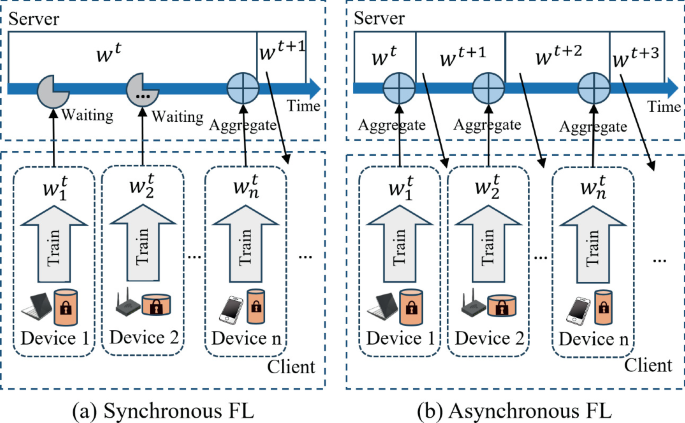
\includegraphics[width=0.9\textwidth]{5.png} % Replace with actual figure
    \caption{Synchronous vs Asynchronous Federated Learning}
    \label{fig:workflow}
\end{figure}

\subsection{Training Variants}

\textbf{1. Synchronous FL}
\begin{itemize}
    \item All selected clients finish training before aggregation
    \item More stable, but slower
\end{itemize}

\textbf{2. Asynchronous FL}
\begin{itemize}
    \item Server updates whenever a client sends updates
    \item Faster but less stable
\end{itemize}

\begin{figure}[H]
    \centering
    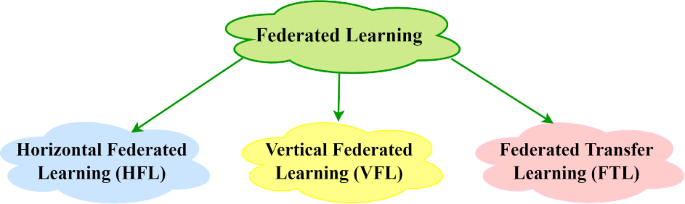
\includegraphics[width=0.9\textwidth]{6.png} % Replace with actual figure
    \caption{Types of Federated Learning}
    \label{fig:sync_async}
\end{figure}

\section{Types of Federated Learning}
\label{sec:types}

\begin{figure}[H]
    \centering
    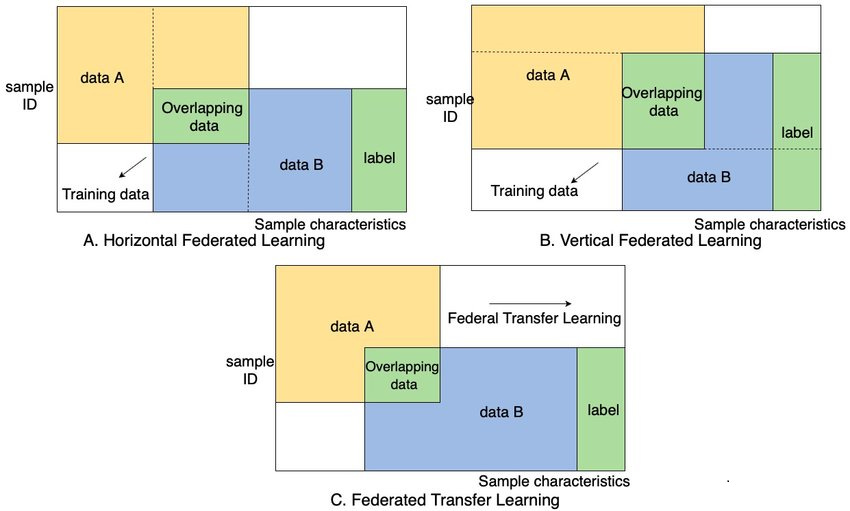
\includegraphics[width=0.9\textwidth]{7.png} % Replace with actual figure
    \caption{Horizontal, Vertical, and Transfer Federated Learning}
    \label{fig:classification}
\end{figure}

\subsection{Horizontal Federated Learning}
\begin{itemize}
    \item Same feature space, different users
    \item \textbf{Example:} Mobile keyboards across users
\end{itemize}

\subsection{Vertical Federated Learning}
\begin{itemize}
    \item Same users, different features
    \item \textbf{Example:} Bank + e-commerce sharing encrypted features
\end{itemize}

\subsection{Federated Transfer Learning}
\begin{itemize}
    \item Different users + different features
    \item Uses transfer learning techniques
\end{itemize}

\section{Privacy Techniques}
\label{sec:privacy}

Federated learning is privacy-preserving, but not perfectly private. It often combines:

\begin{enumerate}
    \item \textbf{Differential Privacy:} Adds noise to updates to prevent reconstruction of data.
    \item \textbf{Secure Aggregation:} Server only sees the \textbf{sum of updates}, not individual ones.
    \item \textbf{Homomorphic Encryption:} Allows computation on encrypted data.
\end{enumerate}

\section{Optimization Challenges}
\label{sec:challenges}

\subsection{Non-IID Data}
Data across clients is \textbf{not identically distributed}.
\begin{itemize}
    \item Example: Different typing styles, different medical records
    \item Causes instability in training
\end{itemize}

\subsection{Unbalanced Data}
Some clients have more data than others.

\subsection{System Heterogeneity}
Devices vary in:
\begin{itemize}
    \item CPU power
    \item Battery
    \item Connectivity
\end{itemize}

\subsection{Communication Bottleneck}
Sending model updates is expensive, especially for large models.

\section{Advanced Techniques}
\label{sec:advanced}

\subsection{Gradient Compression}
Reduces communication size via:
\begin{itemize}
    \item Quantization
    \item Sparsification
\end{itemize}

\subsection{Personalization}
\begin{itemize}
    \item Global model + local fine-tuning
    \item Each client adapts model to its data
\end{itemize}

\subsection{Meta Learning in FL}
Learn a model that can quickly adapt to each client.

\subsection{Federated Averaging Variants}
\begin{itemize}
    \item FedProx: handles non-IID data better
    \item Scaffold: reduces client drift
\end{itemize}

\section{Real-World Applications}
\label{sec:applications}

\subsection{Healthcare}
Hospitals collaboratively train models without sharing patient data.

\subsection{Finance}
Banks detect fraud without exposing sensitive customer data.

\subsection{Mobile Devices}
\begin{itemize}
    \item Predictive keyboards
    \item Voice recognition
    \item Next-word prediction
\end{itemize}

\subsection{Real-Life Application of Federated Learning: Google Keyboard}
\begin{itemize}
    \item \textbf{Data Collection:} Google Keyboard (Gboard) collects data, like the names of restaurants you search for, but keeps it on your phone. Your personal data never leaves your device.
    \item \textbf{Federated Learning in Action:} The model is trained directly on your phone using the data (like your search history). No need to send your data to a central server, keeping it private.
    \item \textbf{Model Updates:} After training locally, the updates to the model are sent to a central server in an encrypted form. The server combines updates from different devices to improve the model.
    \item \textbf{Better Suggestions:} As more updates are gathered, the model gets better at suggesting things, like more accurate restaurant names or typing predictions based on your habits.
    \item \textbf{Privacy and Efficiency:} Your data stays private, and only model updates are shared. This helps save bandwidth and makes everything run more efficiently.
\end{itemize}

\section{Security Risks}
\label{sec:security}

Even though data isn't shared, attacks are still possible:
\begin{enumerate}
    \item \textbf{Gradient Leakage:} Attackers may reconstruct data from gradients.
    \item \textbf{Poisoning Attacks:} Malicious clients send fake updates to corrupt the model.
    \item \textbf{Inference Attacks:} Infer whether a data point was part of training.
\end{enumerate}

\section{Advantages of Federated Learning}
\label{sec:advantages}

\begin{itemize}
    \item \textbf{Reduced Power Usage:} Reduced data size means reduced computation time and hence less power usage.
    \item \textbf{Guarantees Privacy:} Data stays on the device, maintaining privacy without loss of training.
    \item \textbf{No Device Performance Impact:} Training is done only when the device is in idle or charging state, hence no impact on performance.
    \item \textbf{Scalability:} Scales with big, distributed datasets across multiple devices.
    \item \textbf{Better Model Performance:} Uses heterogeneous data from various devices to improve model accuracy.
    \item \textbf{Real-time Updates:} Allows real-time model updates on each device.
\end{itemize}

\section{Disadvantages of Federated Learning}
\label{sec:disadvantages}

\begin{itemize}
    \item \textbf{Network Latency:} The communication between the devices and the central server can be a bottleneck and may add latency to the training process.
    \item \textbf{Heterogeneous devices:} The devices can be heterogeneous in terms of hardware and software, which can make it difficult to ensure the compatibility and consistency of the models.
    \item \textbf{Data Quality:} The quality of data can vary across the devices, which can lead to poor model performance.
\end{itemize}

\section{References}
\label{sec:references}

\begin{enumerate}
    \item \url{https://cloud.google.com/discover/what-is-federated-learning}
    \item \url{https://www.researchgate.net/figure/Classification-of-federated-learning-in-10-a-Horizontal-federated-learning-HFL_fig1_378809686}
    \item \url{https://onlinelibrary.wiley.com/doi/10.1155/2021/8261663}
    \item \url{https://www.youtube.com/watch?v=89BGjQYA0uE}
    \item \url{https://www.geeksforgeeks.org/machine-learning/collaborative-learning-federated-learning/}
    \item \url{https://media.springernature.com/lw685/springer-static/image/chp\%3A10.1007\%2F978-981-95-3543-9_21/MediaObjects/654870_1_En_21_Fig1_HTML.png}
    \item \url{https://media.springernature.com/lw685/springer-static/image/art\%3A10.1007\%2Fs10115-024-02257-6/MediaObjects/10115_2024_2257_Fig8_HTML.png}
\end{enumerate}

\end{document}